\documentclass[conference,12pt]{IEEEtran}
\IEEEoverridecommandlockouts
% The preceding line is only needed to identify funding in the first footnote. If that is unneeded, please comment it out.
\usepackage{amsmath,amssymb,amsfonts}
\usepackage{graphicx}
\usepackage{textcomp}
\usepackage{xcolor}
\usepackage[utf8]{inputenc}
\usepackage[english]{babel}
\usepackage{multicol}
\usepackage{wrapfig}
\usepackage{subfigure}
\usepackage{amssymb}
\usepackage{ wasysym }
\usepackage[]{algorithm}
\usepackage[noend]{algpseudocode}
\graphicspath{ {./images/} }

\usepackage[english]{babel}


\begin{document}

\title{\textbf{Linear Temporal Logic for Robot Path Planning}}
\author{De Filippis Stefano}

\maketitle

\section*{Introduction}

Generally the path planning for a robotic system can be approached by the use of the Geometric A*. The problem is to move on a plane from a starting position to a goal, while avoiding all the obstacles or following some other criteria. 

With the previous mentioned method, the plane is usually discretized with a cell decomposition and we have a state for each point on the grid where allowed moves are only the grid’s lines and diagonal move inside a cell. In this way, though, real optimal path may become impossible since the discretization may make the optimal path longer or the occluded area are not correctly represented in the grid and they may occupy larger areas, resulting in the infeasibility of some path.

With the approach implemented, instead, the problem of robot motion planning is solved by satisfying formulas expressible in temporal logics. Temporal logics naturally express traditional robot specifications such as reaching a goal or avoiding an obstacle, but also more sophisticated specifications such as sequencing, coverage, or temporal ordering of different tasks. 

Also in this case we need to abstract the task by by partitioning the environment into a finite number of equivalence classes, but the resulting discretization will actually be less restraining than the grid decomposition. Then a transition model can be derived from this discretization and so model checking can be used in order to find a trace that satisfies a particular LTL formula encoding the planning goal. Finally, a smoothing procedure is implemented in order to shorten the obtain plan.

\section{Problem Formulation}

If we consider a fully actuated, planar model of robot motion operating in a polygonal environment P, its motion can be expressed as

\begin{equation}
\dot{x} = u(t) \quad x(t) \in P \subseteq \mathbb{R}^2 \quad u(t) \in U \subseteq \mathbb{R}^2
\end{equation}

where $x(t)$ is the position of the robot at time $t$, and $u(t)$ is the control input. The goal is to construct
a control input so that the resulting trajectory $x(t)$ satisfies a LTL formula.

The formulas are built from a finite number of atomic propositions or observables which label areas of interest in the environment such as rooms or obstacles. Let $\Pi = \{ \pi_1, \pi_2,..., \pi_n \}$ be a set of such propositions. For the previous system we then associate an observation map

\begin{equation}
h_C : P \rightarrow \Pi
\end{equation}

which maps the continuous states of the robot to the finite set of propositions. Proposition $\pi_i \in \Pi$ represents an area of interest in the environment which can be characterized by a convex set of the form:

\begin{equation}
P_i = \{x \in \mathbb{R}^2|\bigwedge_{1 \leq k \leq m}a_k^Tx+b_k \leq 0, a_k \in \mathbb{R}^2,b_k \in \mathbb{R}^2 \}
\end{equation}

All the previous relations simply state that the observation map $h_C : P \rightarrow \Pi$ has the form $h_C(x) = \pi_i$ iff $x$ belongs in the associated set $P_i$.

Therefore, Given the robot model, the observation map, the initial condition $x(0) \in P$ , and a LTL temporal logic formula $\phi$,  the problem is to construct a control input $u(t)$ so that the resulting robot trajectory $x(t)$ satisfies the formula.

\section{Linear Temporal Logic}

Propositional logic is the traditional logic of conjunction ($\wedge$), disjunction ($\vee$), negation ($\neg$), implication ($\Rightarrow$), and equivalence ($\Leftrightarrow$). LTL is obtained from standard propositional logic by adding temporal operators such as eventually ($\Diamond$), always ($\Box$), next ($\ocircle$) and until ($\mathcal{U}$).

Some LTL examples that express interesting properties include:

\begin{itemize}
\item Reach goal while avoiding obstacles is expressed by the formula: $\neg(o_1 \vee o_2 \vee ... \vee o_n) \mathcal{U} \pi$
\item A sequencing requiremente can be encoded with $\Diamond( \pi_i \wedge \Diamond ( \pi_j \wedge ( ... \Diamond ( \pi_k \wedge \Diamond \pi_l) )))$
\item a coverage properties instead is represented by: $\Diamond \pi_i \wedge \Diamond \pi_j \wedge ... \wedge \Diamond \pi_k$
\end{itemize}

\section{LTL Motion Planning}

So in order to solve the previously defined problem we need to execute the 2 following steps:

\begin{enumerate}
\item Discrete Abstraction of Robot Motion: Decompose the environment P into a finite number of equivalence classes resulting in a finite state model of robot motion.
\item Temporal Logic Planning using Model Checking: Construct plans for the discrete robot motion satisfying desired specifications using model checkers.
\end{enumerate}

\subsection{Discrete Abstraction of Robot Motion}

I first need to partition the workspace P of the robot into a finite number of equivalence classes and for my experiments I used the Delaunay Triangulation which is well implemented in matlab and a very efficient technique to partition complex environment.

Let $T : P \rightarrow Q$ denote the map which sends each state $x \in P$ to the finite set $Q = \{q_1 , . . . , q_n \}$ of all equivalence classes (triangles in my case). In other words, $T^{-1}(q)$ contains all states $x \in P$ which are contained in the triangle labeled by $q$ and $\{T^{-1}(q_i) | q_i \in Q\}$ is a partition of the state space. Given such a partition of $P$ , we can naturally abstract the robot motion by defining a finite transition system

\begin{equation}
D = (Q,q(0) \rightarrow_D,h_D)
\end{equation}

where $Q$ is the finite set of states, and $q(0) \in Q$ is the cell containing the initial robot state $x(0) \in P$ , that is $q(0) = T(x(0))$. The dynamics are captured by the transition relation $\rightarrow_D \subseteq Q \times Q$, defined as $q_i \rightarrow_D q_j $ iff the cells labeled by $q_i$ , $q_j$ are topologically adjacent, that is triangles $T^{-1}(q_i)$ and $T^{-1}(q_j)$ have a common line segment. The transition relation $\rightarrow_D$ is also known as the dual graph of the triangulation and can be easily computed.

Having defined transitions $\rightarrow_D$ for transition system $D$, we can define trajectories $p$ of $D$ as sequences of the form $p[i] = p _i \rightarrow_D p_{i+1} \rightarrow_D p_{i+2} \rightarrow_D . . .$ , where $p_i = p(i) \in Q$. In addition to defining the transition relation, we also define the observation map $h_D : Q \rightarrow \Pi$, as $h_D(q) = \pi$, if there exists $x \in T^{-1}(q)$ such that $h_C(x) = \pi$.

In order to ensure that $h_D$ is well defined, we must impose the requirement that the decomposition is proposition or observation preserving, that is for all $x_1 , x_2 \in P$ and all $\pi \in \Pi, T(x _1) = T(x_2) \Rightarrow h_C(x_1 ) = h_C(x_2)$. In other words, states that belong in the same equivalence class or cell, map to the same observations.

The transition system $D$ will serve as an abstract model of robot motion. We must now lift our problem formulation from the continuous to the discrete domain and we reformulate the semantics of the temporal logic formula to be interpreted over the discrete trajectories generated by transition system $D$.

Path formulas $\phi$ are interpreted over an execution $p[i]$, denoted as $p[i] \models_D \phi$. The semantics of any path formula can be recursively defined as:

\begin{itemize}
\item $p[i] \models_D \pi$ iff $h_D(p(i)) = \pi$
\item $p[i] \models_D \neg \phi$ if $p[i] \nvDash_D \phi$
\item $p[i] \models_D \phi_1 \vee \phi_2$ if $p[i]  \models_D \phi_1$ or $p[i] \models_D \phi_2$
\item $p[i] \models_D \phi_1 \mathcal{U} \phi_2$ if there exists $j \geq i$ s.t. $p[j] \models_D \phi_2$ , and for all $j'$ with $i \leq j' < j $ we have $p[j'] \models_D \phi_1$
\end{itemize}

\subsection{Temporal Logic Planning using Model Checking}

Model checking is the algorithmic procedure for testing whether a specification formula holds over some semantic model. The model of the system is usually given in the form of a discrete transition system like the one described previously. The specification formula is usually given in the form of temporal logics such as LTL. 

As mentioned earlier, we are looking for computation
paths $p[i]$ that satisfy the temporal formula $p[0] \models_D \phi$ and in practice we want to generate atrace of witnesses that satisfy the formula. Unfortunately, the current versions of the model checking software tools do not support the construction of witnesses as they are mainly analysis tools. Hence, we have to employ the algorithms that solve the dual problem, i.e. the generation of counterexamples.

In this case, when the model checker determines that a formula $\phi$ is false, it constructs a finite trace $p[0]$ which demonstrates that the negation of $\phi$ is true, i.e. $p[0] \models_D \neg \phi$. Let $\phi$ be the formula that the system should satisfy. Assume now that we give as input to our model checking algorithm the LTL formula $\neg \phi$, representing the negation of the desired behavior. If the formula is false in our discrete model of the environment, then the model checker will return a finite trace $p[0]$ that satisfies the formula $\neg(\neg \phi)\equiv \phi$ and, thus, we are done as we have found a finite path that satisfies the original LTL formula $\phi$.

\section{Implementation}

All the implementation were conducted in MATLAB and NuSMV. In MATLAB I executed all the processing step for the discretization. First I defined all the vertices of the map and the rooms and I used the  delaunay triangulation to get the equivalence classes.

Once I had the triangulation of my environment I used the dual graph in order to build the transition model. In fact, after the triangulation I also have a particular graph whose nodes are the triangles of the decomposition and the edges connects triangles which shares an edge. This means that every node will have at most three edges. Now, from this I can build the transition model in the following way. I build a robot discrete state for each triangle and the transition function follows directly the edges in the dual graph.

The transition model will actually be used in te NuSMV software which will execute the model checking. Therefore, in MATLAB I wrote a simple function which will translate the transition model into a NuSMV input file. In practice in this file I create a single module main and define as boolean the $\pi$ variables which represent the interesting areas in the room and are the predicates that appear in the actual LTL formula. Moreover, I also defined as many variables as nodes in the dual graph. The initial state for the $\pi$ variables depends on where the robot is in the initial state. For the transitions definition, instead, I first write the transition for the discrete robot model: for each state I say that I can undeterministically end up in one of the adjacent state in the dual graph. The transitions for the $\pi$ variables, instead, depend on the actual value of the robot discrete state. In fact, I define that a variable $\pi$ is true if and only if the current robot state is one of the triangle in which the associated room has been decomposed into, otherwise it is set to false.

After creating this input file by also adding the negation of the actual formula I want to satisfy, I start the NuSMV software and launch the model checking on the model. Afterwards I can simply save on an external file the trace found, which will correspond to a set of robot states and therefore a certain number of triangles that have been passed through by the robot, and I build the final trajectory by connecting with straight line the centers of all the visited triangles.

\section{Post Smoothing}

After generating the trajectory I noticed that a lot of intermediate steps could have been avoided in order to obtain a shorter path. Therefore, I decided to modify the paper approach in order to also include a post smoothing procedure.

The algorithm is actually very similar to the one that is used when the Geometric A* is used, but I needed to do some modifications since in some of the rooms/obstacles I can enter. Therefore the algorithm is the following:

\begin{figure*}[t]
	\begin{minipage}{\columnwidth}
		\centering
		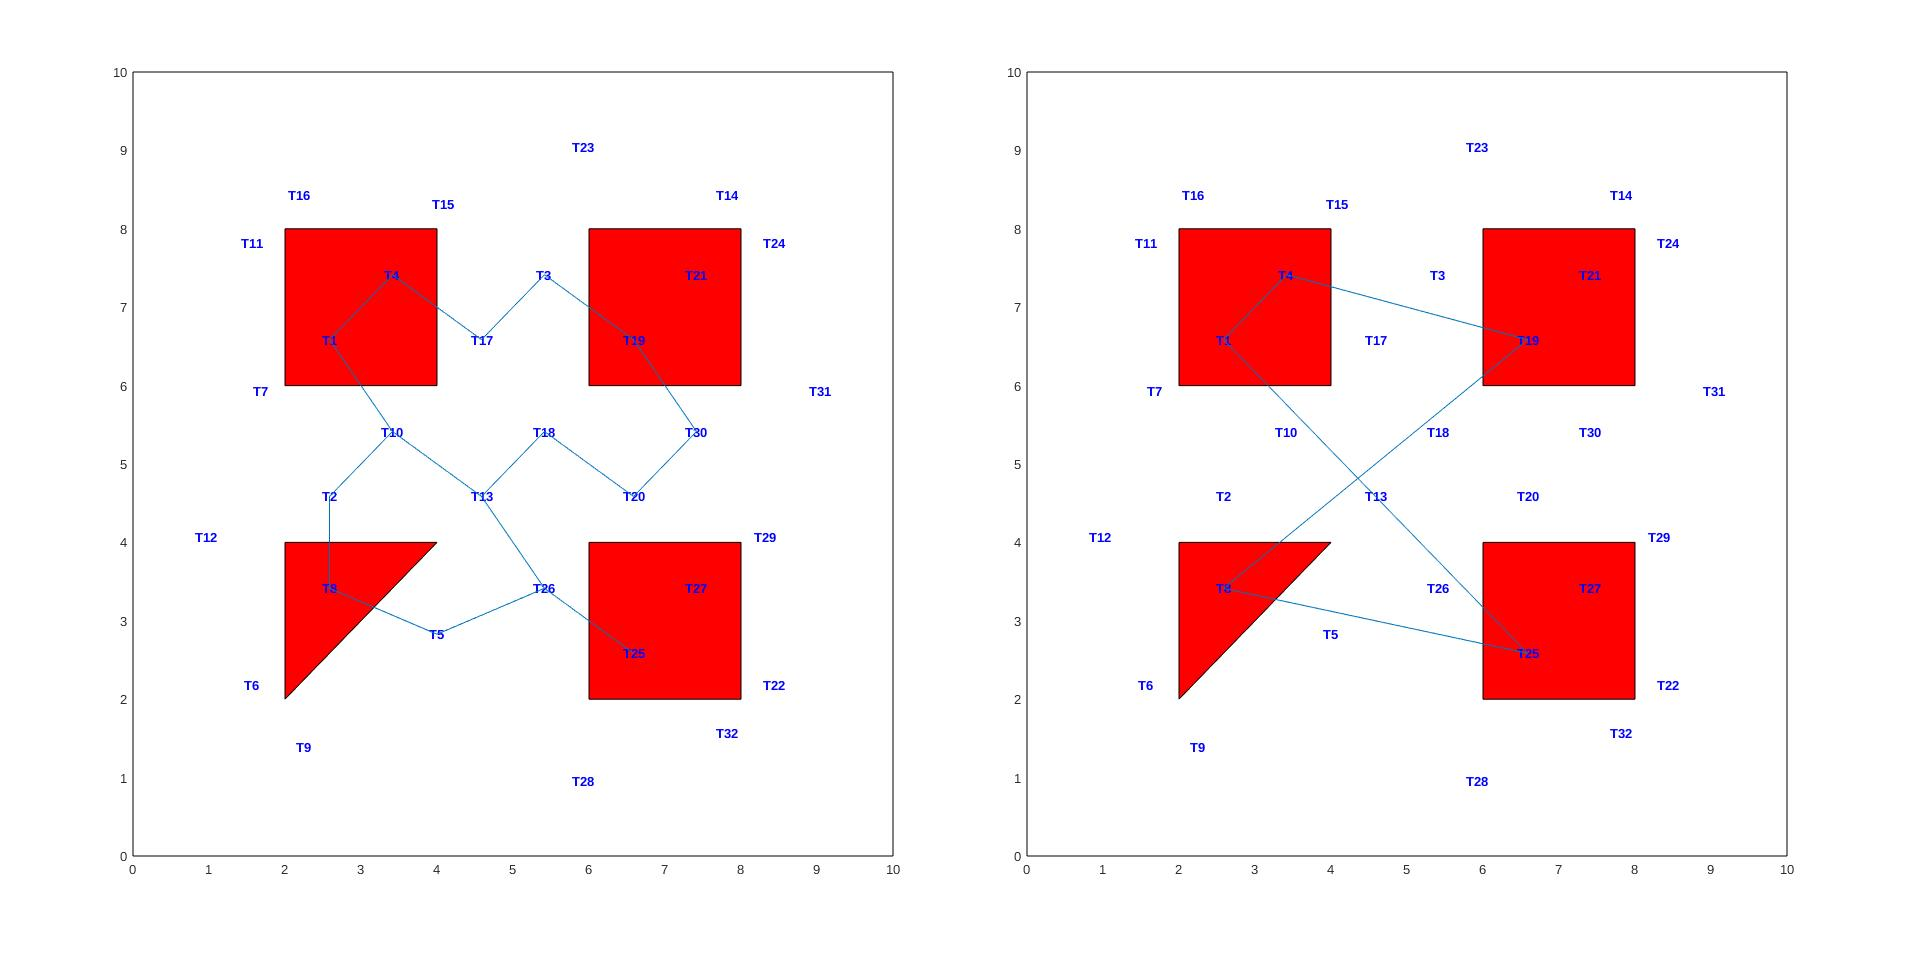
\includegraphics[width=\textwidth]{./1example/path.jpg}
		\caption{First Case}
		\label{first}
	\end{minipage}%
	\begin{minipage}{\columnwidth}
		\centering
		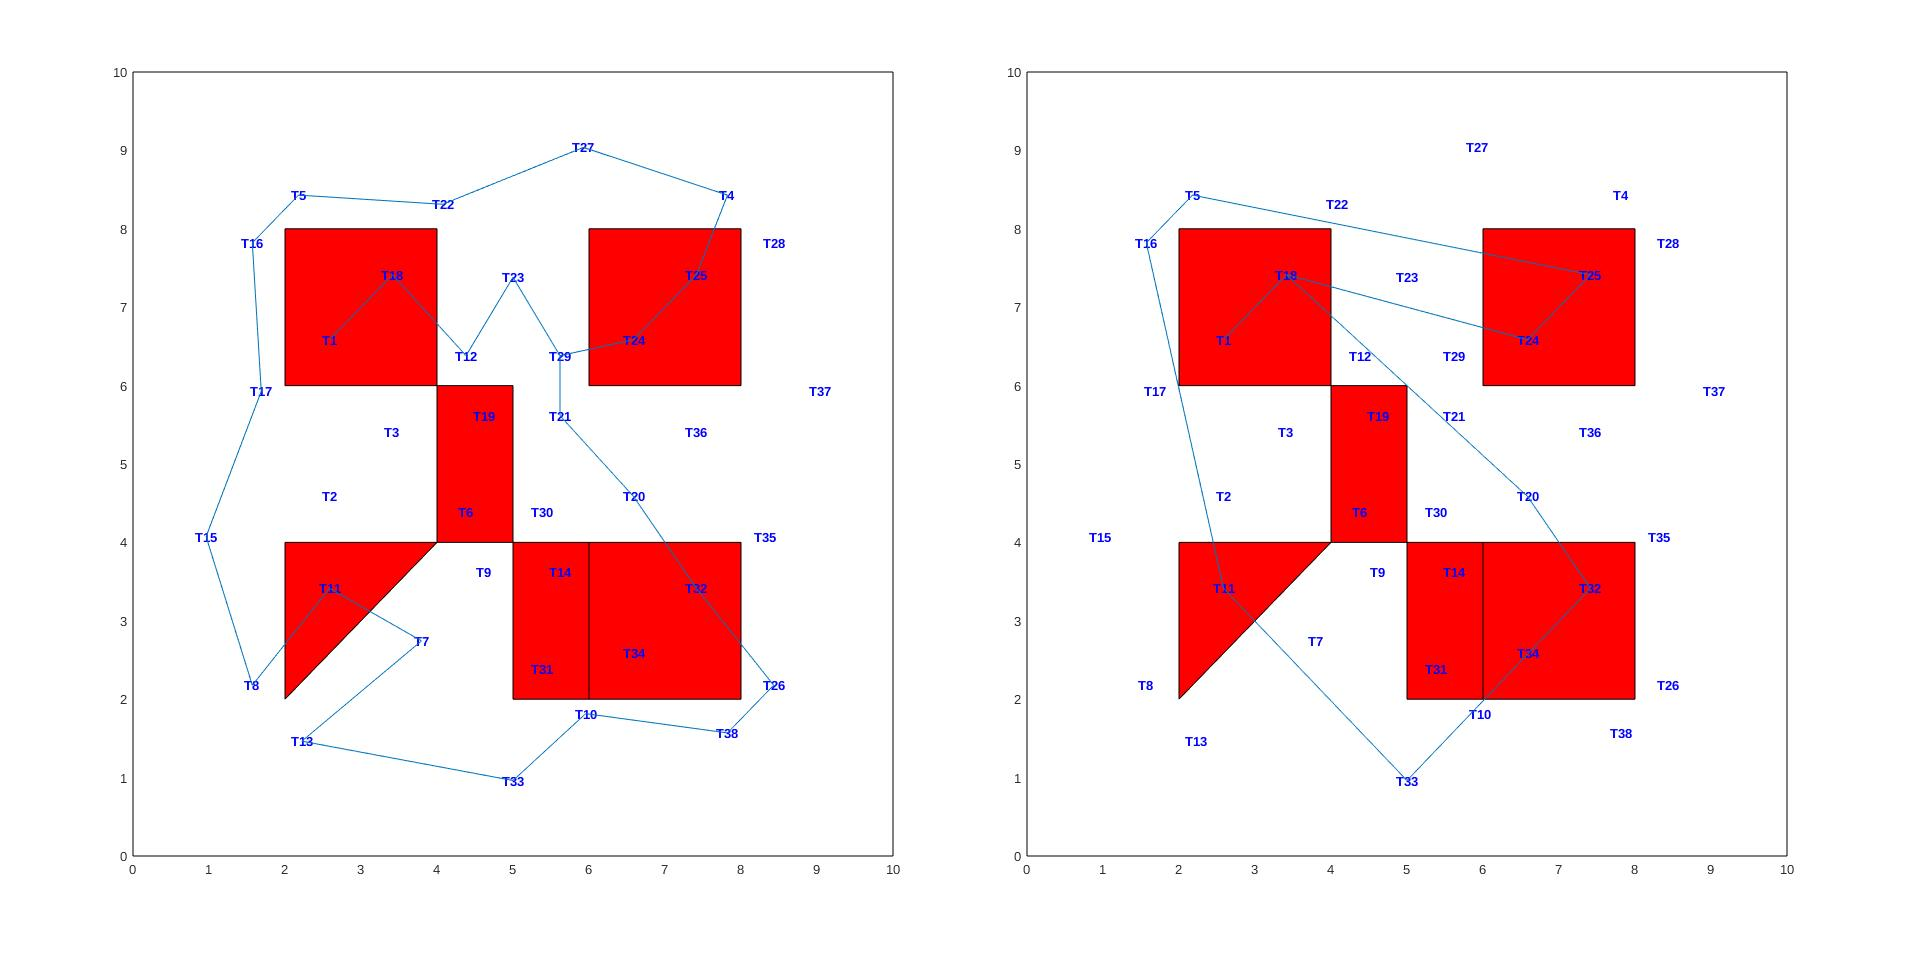
\includegraphics[width=\textwidth]{./2example/path.jpg}
		\caption{Second Case}
		\label{second}
	\end{minipage}
\end{figure*}

\begin{figure*}[t]
\centerline{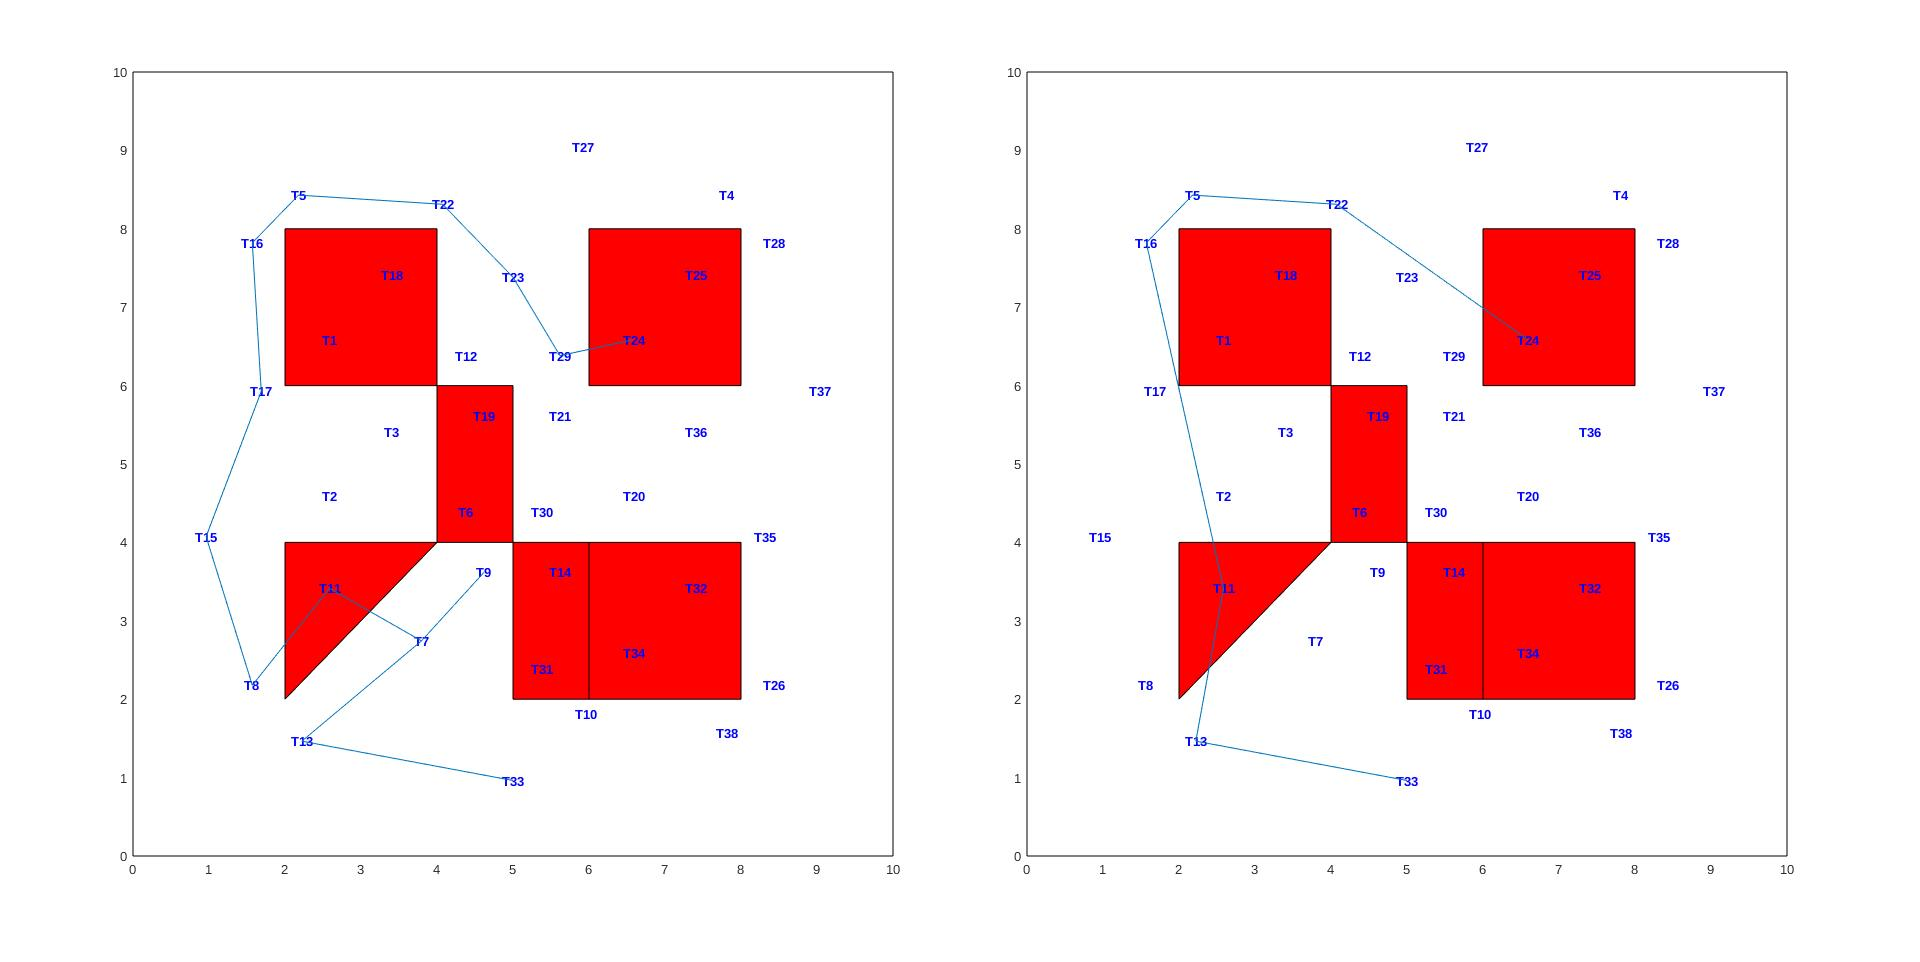
\includegraphics[width=0.5\textwidth]{./4example/path.jpg}}
\caption{Third Case}
\label{third}
\end{figure*}

\begin{algorithm}
\caption{Post Smoothing}\label{euclid}
\begin{algorithmic}[1]
\Procedure{Post Smoothing}{}
\For {\textit{each valid\_state s}}
\State {\textit{valid\_successor} $\gets$ \textit{successor(s)}}
\State {\textit{safe} $\gets$ \textit{True}}
\State {\textit{stop} $\gets$ \textit{False}}
\For {\textit{each successor(s) next and safe not False and stop not True}}
\State {$\textit{line} \gets \textit{segment(s,next)}$}
\For{\textit{ecah room} $\pi$}
\State{\textit{inter} $\gets$ \textit{intersection(line,}$\pi$)}
\If{\textit{inter not 0 and s and next not in} $\pi$}
\State{\textit{safe} $\gets$ \textit{False}}
\EndIf
\If{\textit{inter not 0 and next in} $\pi$}
\State{\textit{stop} $\gets$ \textit{True}}
\EndIf
\EndFor
\If{\textit{safe}}
\State{\textit{valid\_successor} $\gets$ \textit{next}}
\State{\textit{s} $\gets$ \textit{valid\_successor}}
\EndIf
\EndFor
\EndFor
\EndProcedure
\end{algorithmic}
\end{algorithm}

So for each state I try to look at the successor and try to skip them if their successor are in line of sights of the current analyzed state. Some cases, though, are particular. 

First, when I am checking if the line between two states intersect any room in the environment, I need to check if the current state is inside the room. In this case the intersection is allowed since I need to pass through that the room because the starting point is inside it and therefore the analyzed successor is still a valid candidate. 

Instead, when the intersection is with a room where neither the current state or the successor is in, then this means that I am passing through some obstacle and so I stop to the previous validate candidate and start the new checks from there. 

Finally, if the intersection is with a room where the current successor is in, then this is still a valid candidate but I need to stop the search, otherwise I could find other valid successors and skip the passage through this particular room.

\section{Experiments}

In the following section I will report the experiments I conducted in order to validate the method.

\subsection{First Case}

First I tried to only include 4 rooms in the environment and the robot needed to start from room 1 and visit with the particular order the room 2, 3 and 4 and finally return back to the first room while avoiding the room 2 and 3.

The Formula that correctly represents this requirements is:

\begin{equation}
\Diamond(\pi_2 \wedge \Diamond(\pi_3 \wedge \Diamond(\pi_4 \wedge (\neg \pi_2 \wedge \neg \pi_3) \mathcal{U} \pi_1)))
\end{equation}

In Figure \ref{first} we can see the generated path and smoothed version.

\subsection{Second Case}

In the second experiment I added 2 more rooms in the environment and the goal of the robot was to visit in the order the rooms 4, 3, 2 and 1 while always avoiding the rooms 5 and 6.

The formula in this case was:

\begin{equation}
\ocircle (\neg \pi_5 \wedge \neg \pi_6) \wedge \Diamond(\pi_4 \wedge \Diamond(\pi_3 \wedge \Diamond(\pi_2 \wedge \Diamond \pi_1)))
\end{equation}

In Figure \ref{second} we can see the generated path and smoothed version.

\subsection{Third Case}

 Finally with the last experiments I used the previous environment, but I started from the room 2 and wanted to reach the room 3 while avoiding all the other rooms.
 
The correct formulations is encoded by:

\begin{equation}
(\neg \pi_1 \wedge \neg \pi_4 \wedge \neg \pi_5 \wedge \neg \pi_6) \mathcal{U} \pi_3
\end{equation}

In Figure \ref{third} we can see the generated path and smoothed version.

\section{Conclusions}

With this assignment I was able to approach the path planning problem resolution from a different point of view of the standard search in state space algorithm. 

The use of LTL is actually quite effective in order to find a path on a plane and the decomposition used is actually less restrictive than the classical cell decomposition, since we are not constraining movement on the grids or we are not approximating occluded area in wrong ways. 

Still, the resulting path can be sub optimal because a lot of turns are executed, but this can be solved by implementing a simple post smoothing algorithm which takes care of the possibility of entering some rooms in the smoothing process.

\end{document}